\subsubsection{Purpose}
The main purpose of the login feature is to grant the access to the \emph{PowerEnJoy} service to any registered user. The system requires a valid e-mail address and password to login without generating any error.

In addition to that, the login screen offers the chance to recover a forgotten password. The user clicks on \emph{"Forgot password?"}, a new one is sent to his e-mail address immediately and he/she can carry out the login procedure with the new password provided by the system.

\subsubsection{Scenario 1}
Mike would like to rent a car for having a ride in a beautiful sunny day. In order to do that he needs to access the system by means of his credentials. He opens the \emph{PowerEnJoy} home page and enters his e-mail address and his password. Then Mike clicks on \emph{"login"} and, due to the fact that everything is correct, he obtains the access as a logged user.

\subsubsection{Scenario 2}
Bill wants to take the advantage of the \emph{PowerEnJoy} service. He opens the home page and he is asked for his e-mail address and password. He is aware of his e-mail address, but he does not remember the password. After some time spent trying to recall his personal password, Bill inputs his e-mail address and decides to click on \emph{"Forgot password?"}. Right away the system sends a new password to the specified e-mail address. Bill can now enter the system using the new password.

\subsubsection{Use-case}
The login use-case is analyzed in Table \ref{login_uc}.

\subsubsection{Activity diagram}
The login activity diagram is shown in Figure \ref{login_act}.

\subsubsection{Sequence diagram}
The sequence diagram of the login procedure is shown in Figure \ref{login_se}.

\subsubsection{Functional requirements}
\begin{enumerate}
\item The user must be already registered to the system in order to perform a successful login;
\item The user must be aware of his e-mail address and password to successfully obtain the system access;
\item The password provided by the user must correspond to the specified e-mail address;
\item Wrong credentials prevent the user to access the system;
\item The system sends a new password to the specified e-mail address if and only if the specified e-mail address is valid, registered to the system and the user clicks on \emph{"Forgot password?"};
\item After requesting a new password, the system must allow the user login with the new provided password;
\item After three times the entered password is wrong, the system prevents a new attempt for the following 30 seconds;
\item The system must not allow a registered user with a suspended account due to pending payments to log in.
\end{enumerate}

\begin{table}[H]
\begin{center}
\begin{tabular}{p{0.3\textwidth} | p{0.7\textwidth}}
\hline
Actor & Guest\\
\hline
Goal & Goal 1\\
\hline
Input Condition & The guest is already registered to the system and wants to login.\\
\hline
Event Flow & 
\begin{enumerate}
\item The guest opens the \emph{PowerEnJoy} home page or the mobile application and the system shows the login page;
\item The guest enters his/her e-mail address and password;
\item The guest clicks on \emph{"login"} button.
\end{enumerate} \\
\hline
Output Condition & The system lets the guest log in and loads his/her personal home page.\\
\hline
Exception & 
If the e-mail address provided by the guest has never been registered to the system or if the password does not correspond to the entered e-mail, the system notifies the guest with an error message.

If the guest enters wrong credentials three times in a row, the system will prevent any attempt for the following 30 seconds informing him/her.\\
\hline
\end{tabular}
\end{center}
\caption{Login use-case}
\label{login_uc}
\end{table}

\begin{figure}[H]
\begin{center}
		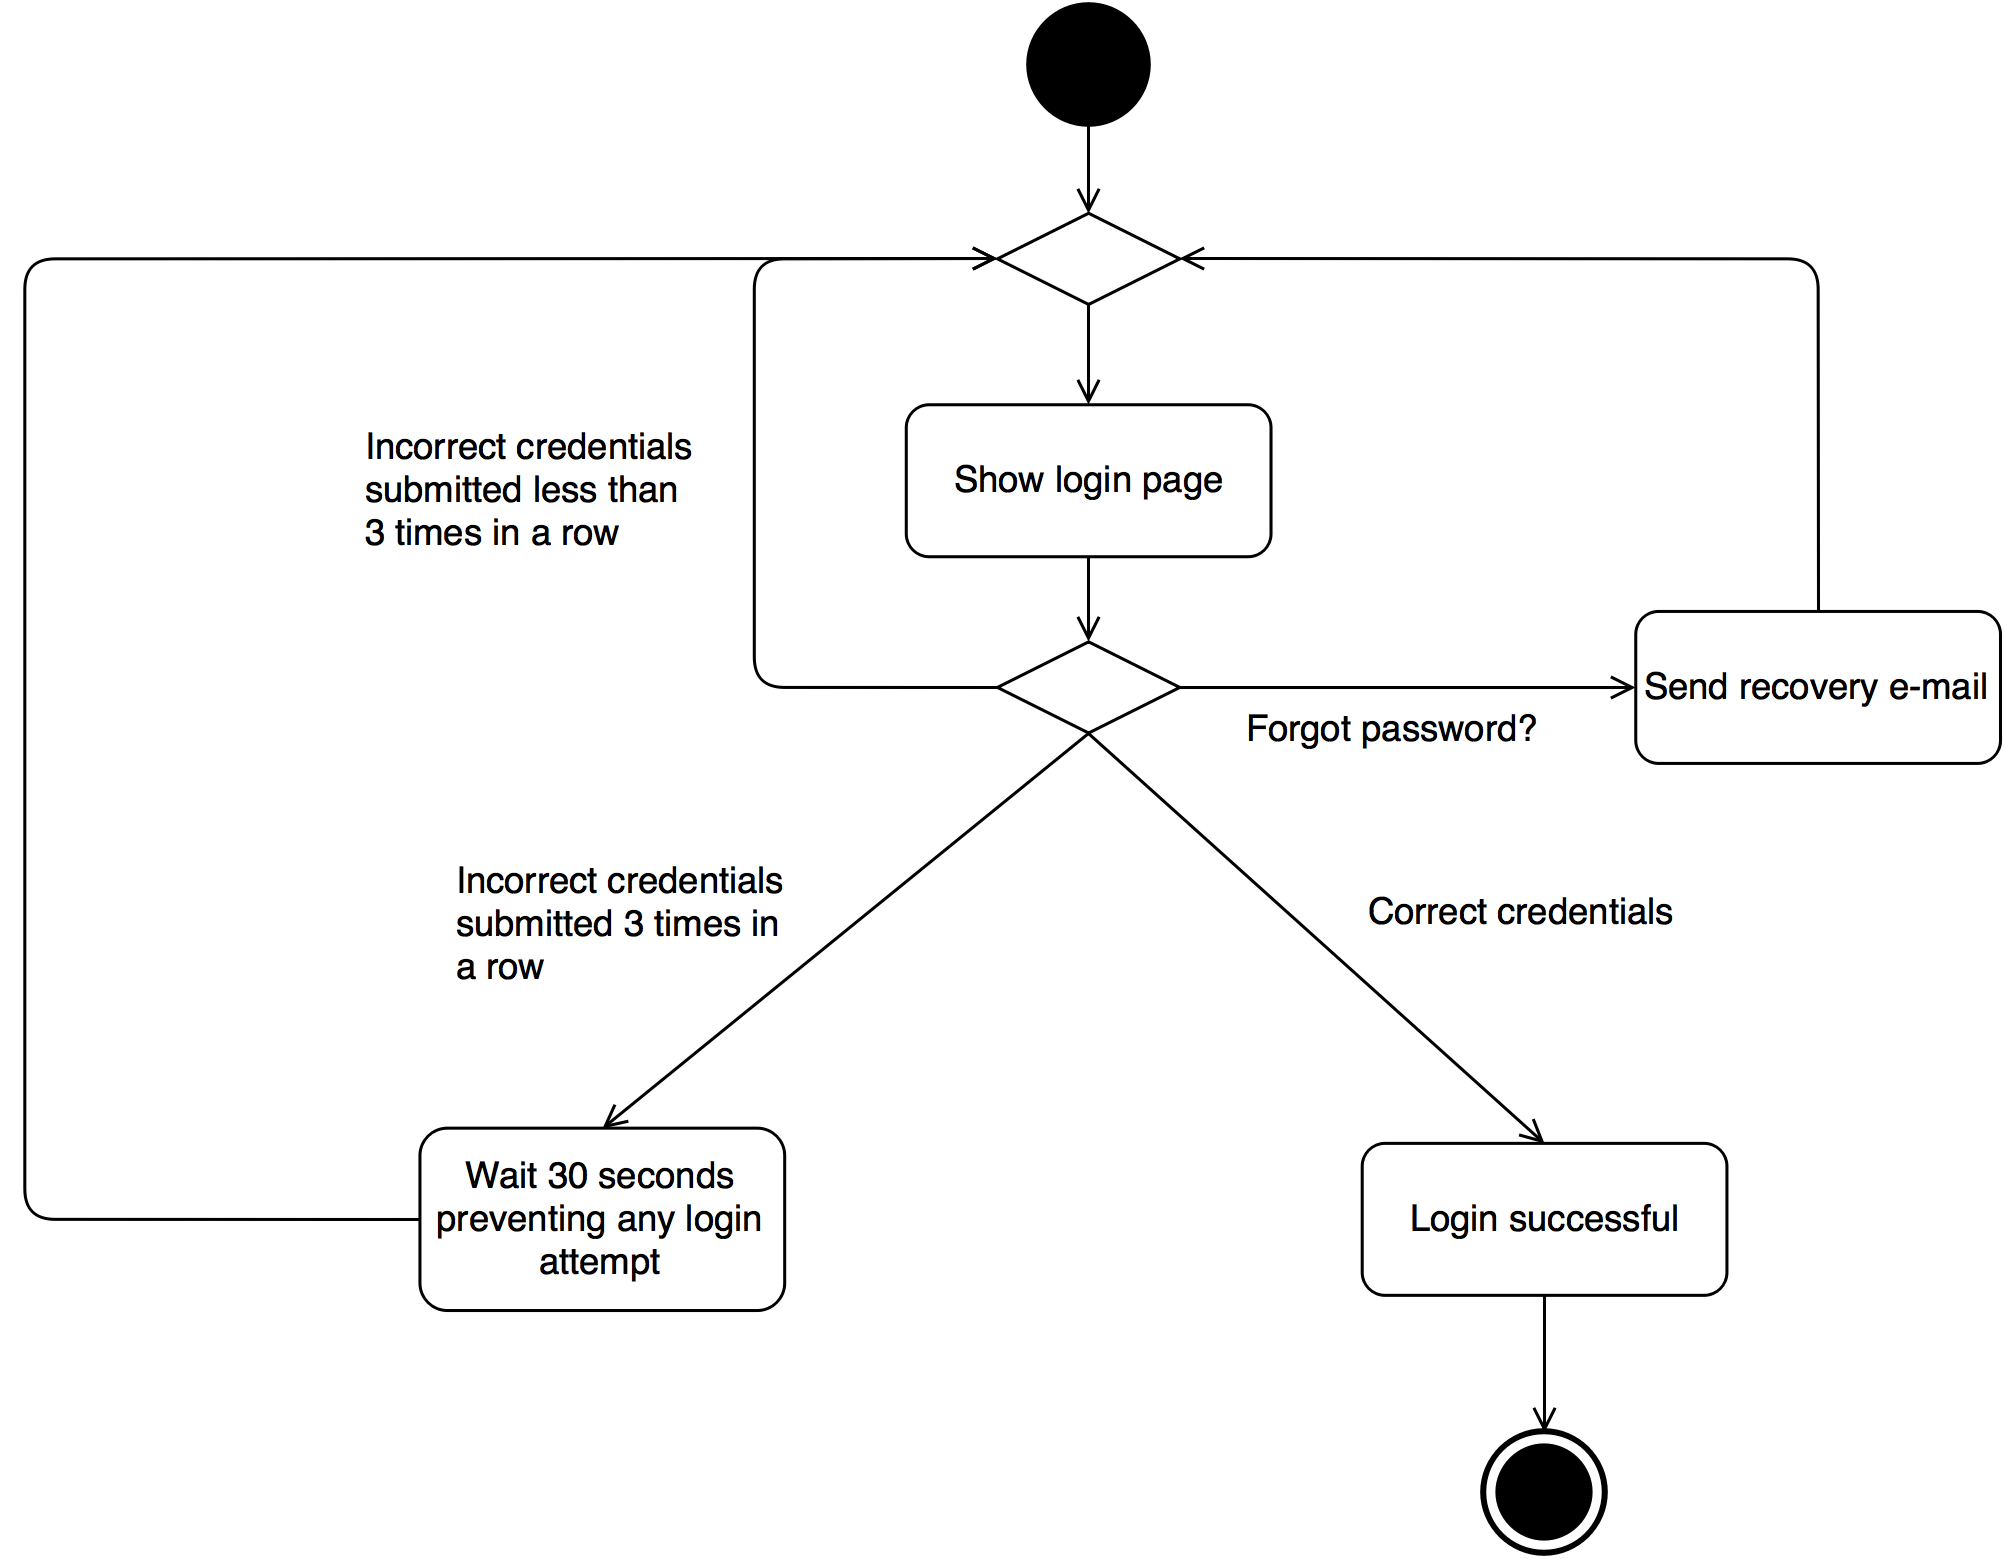
\includegraphics[width=0.8\textwidth]{./specific_requirements/features/diagrams/login_activity.png}
		\caption{Activity diagram of the login process from the system point of view.}
		\label{login_act}
\end{center}
\end{figure}

\begin{figure}[H]
\begin{center}
		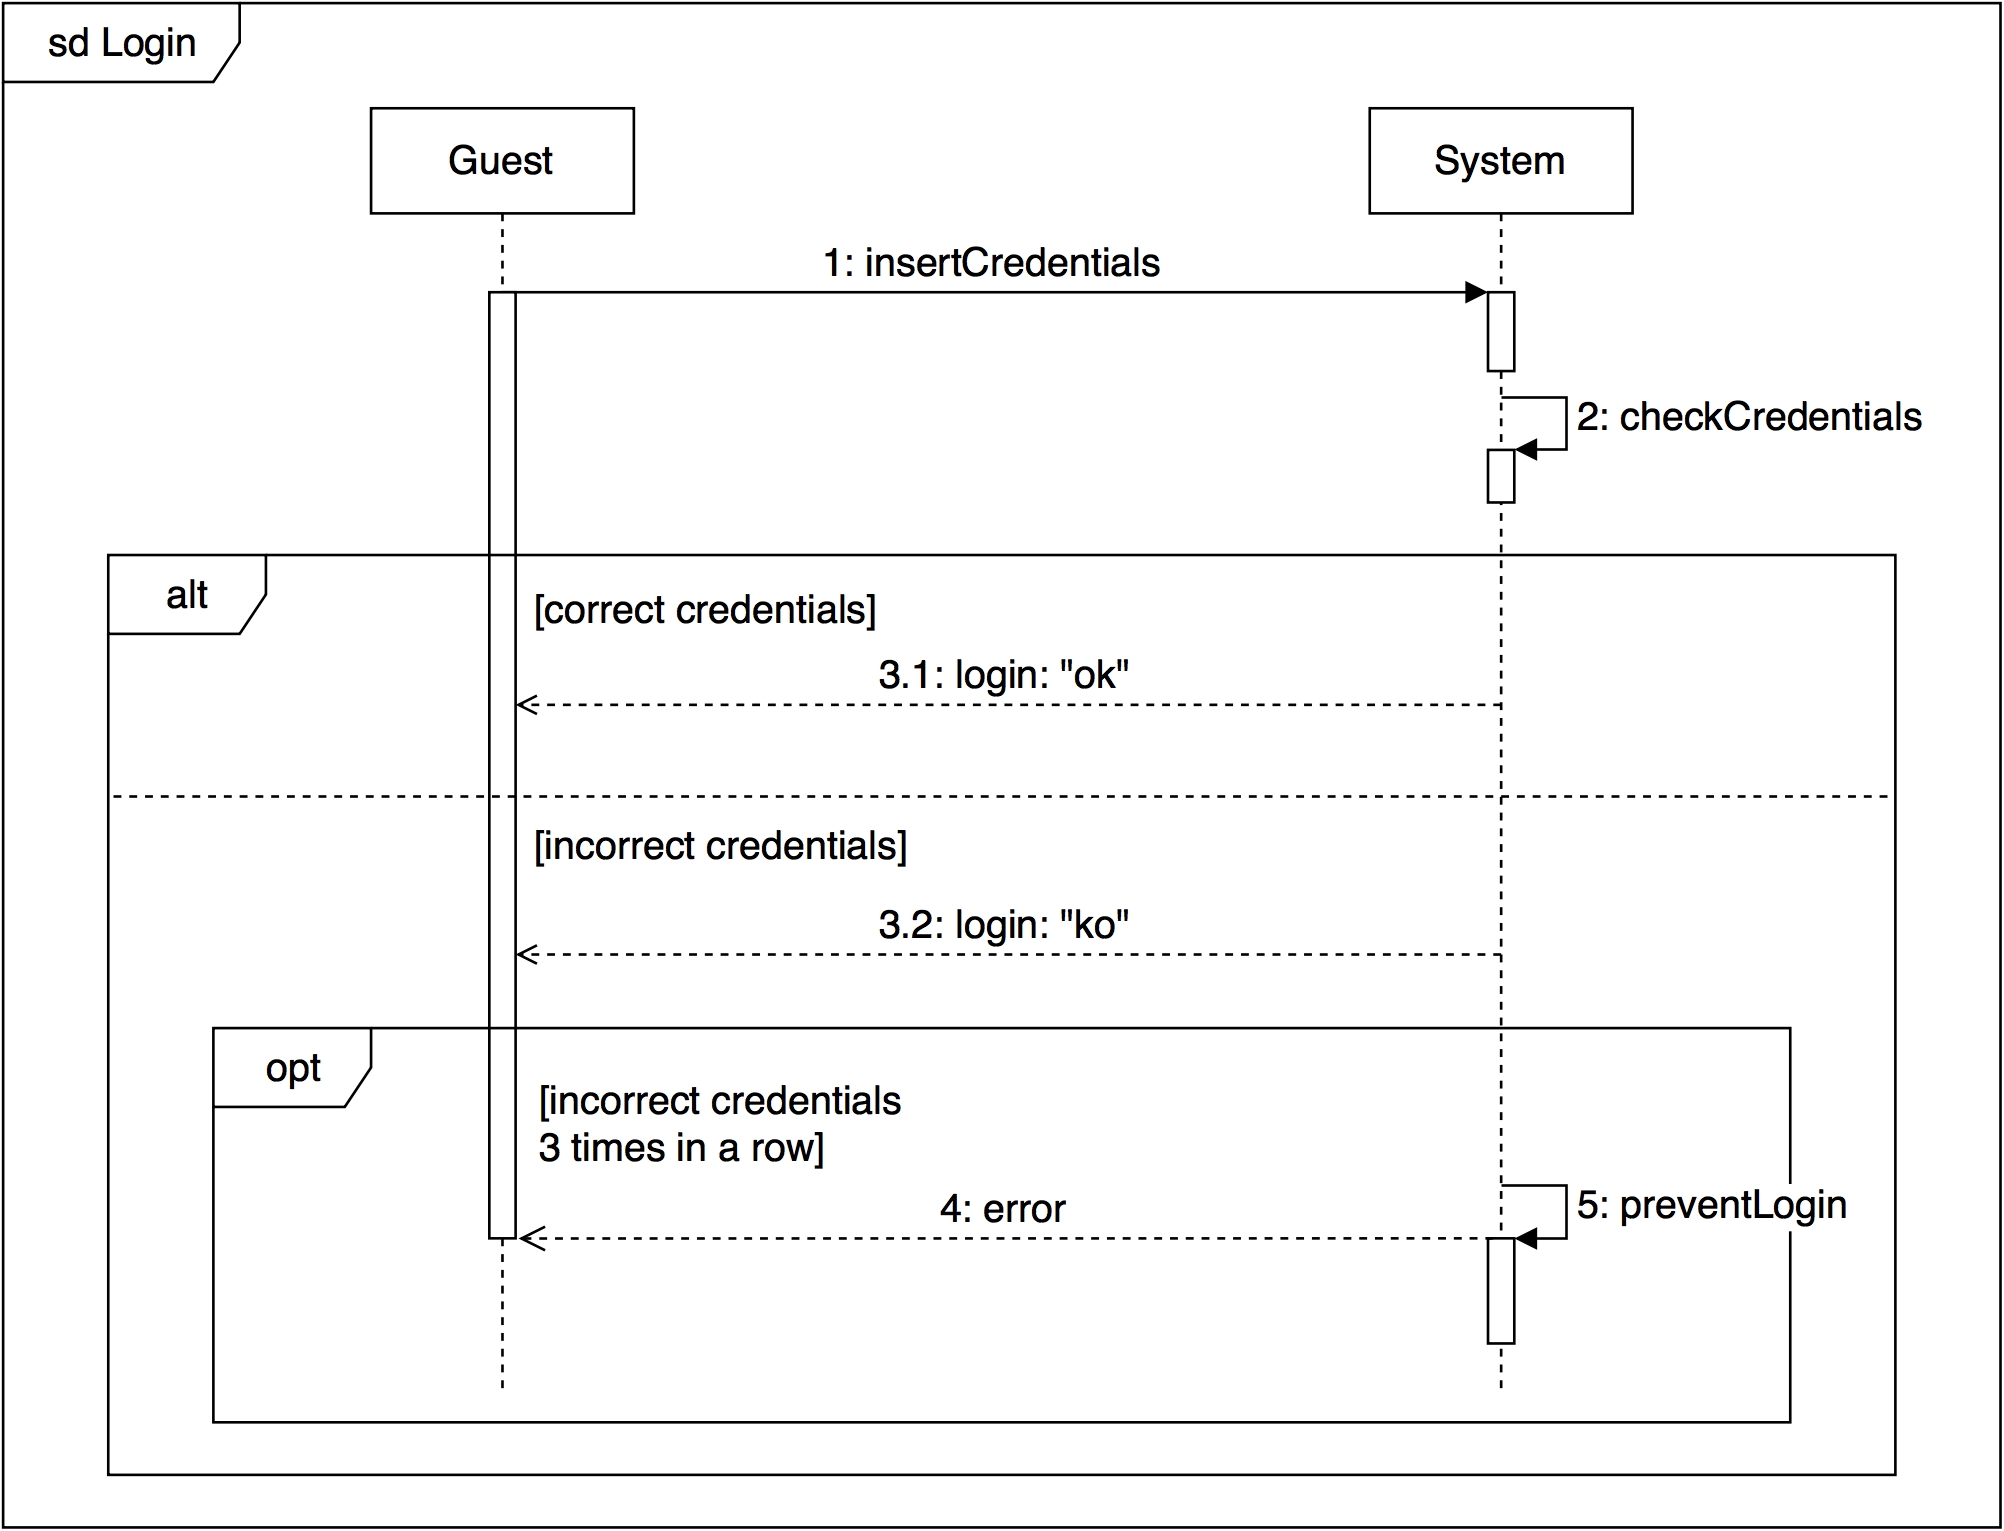
\includegraphics[width=0.8\textwidth]{./specific_requirements/features/diagrams/login_sequence.png}
		\caption{Sequence diagram of the login process.}
		\label{login_se}
\end{center}
\end{figure}

\begin{figure}[H]
\begin{center}
		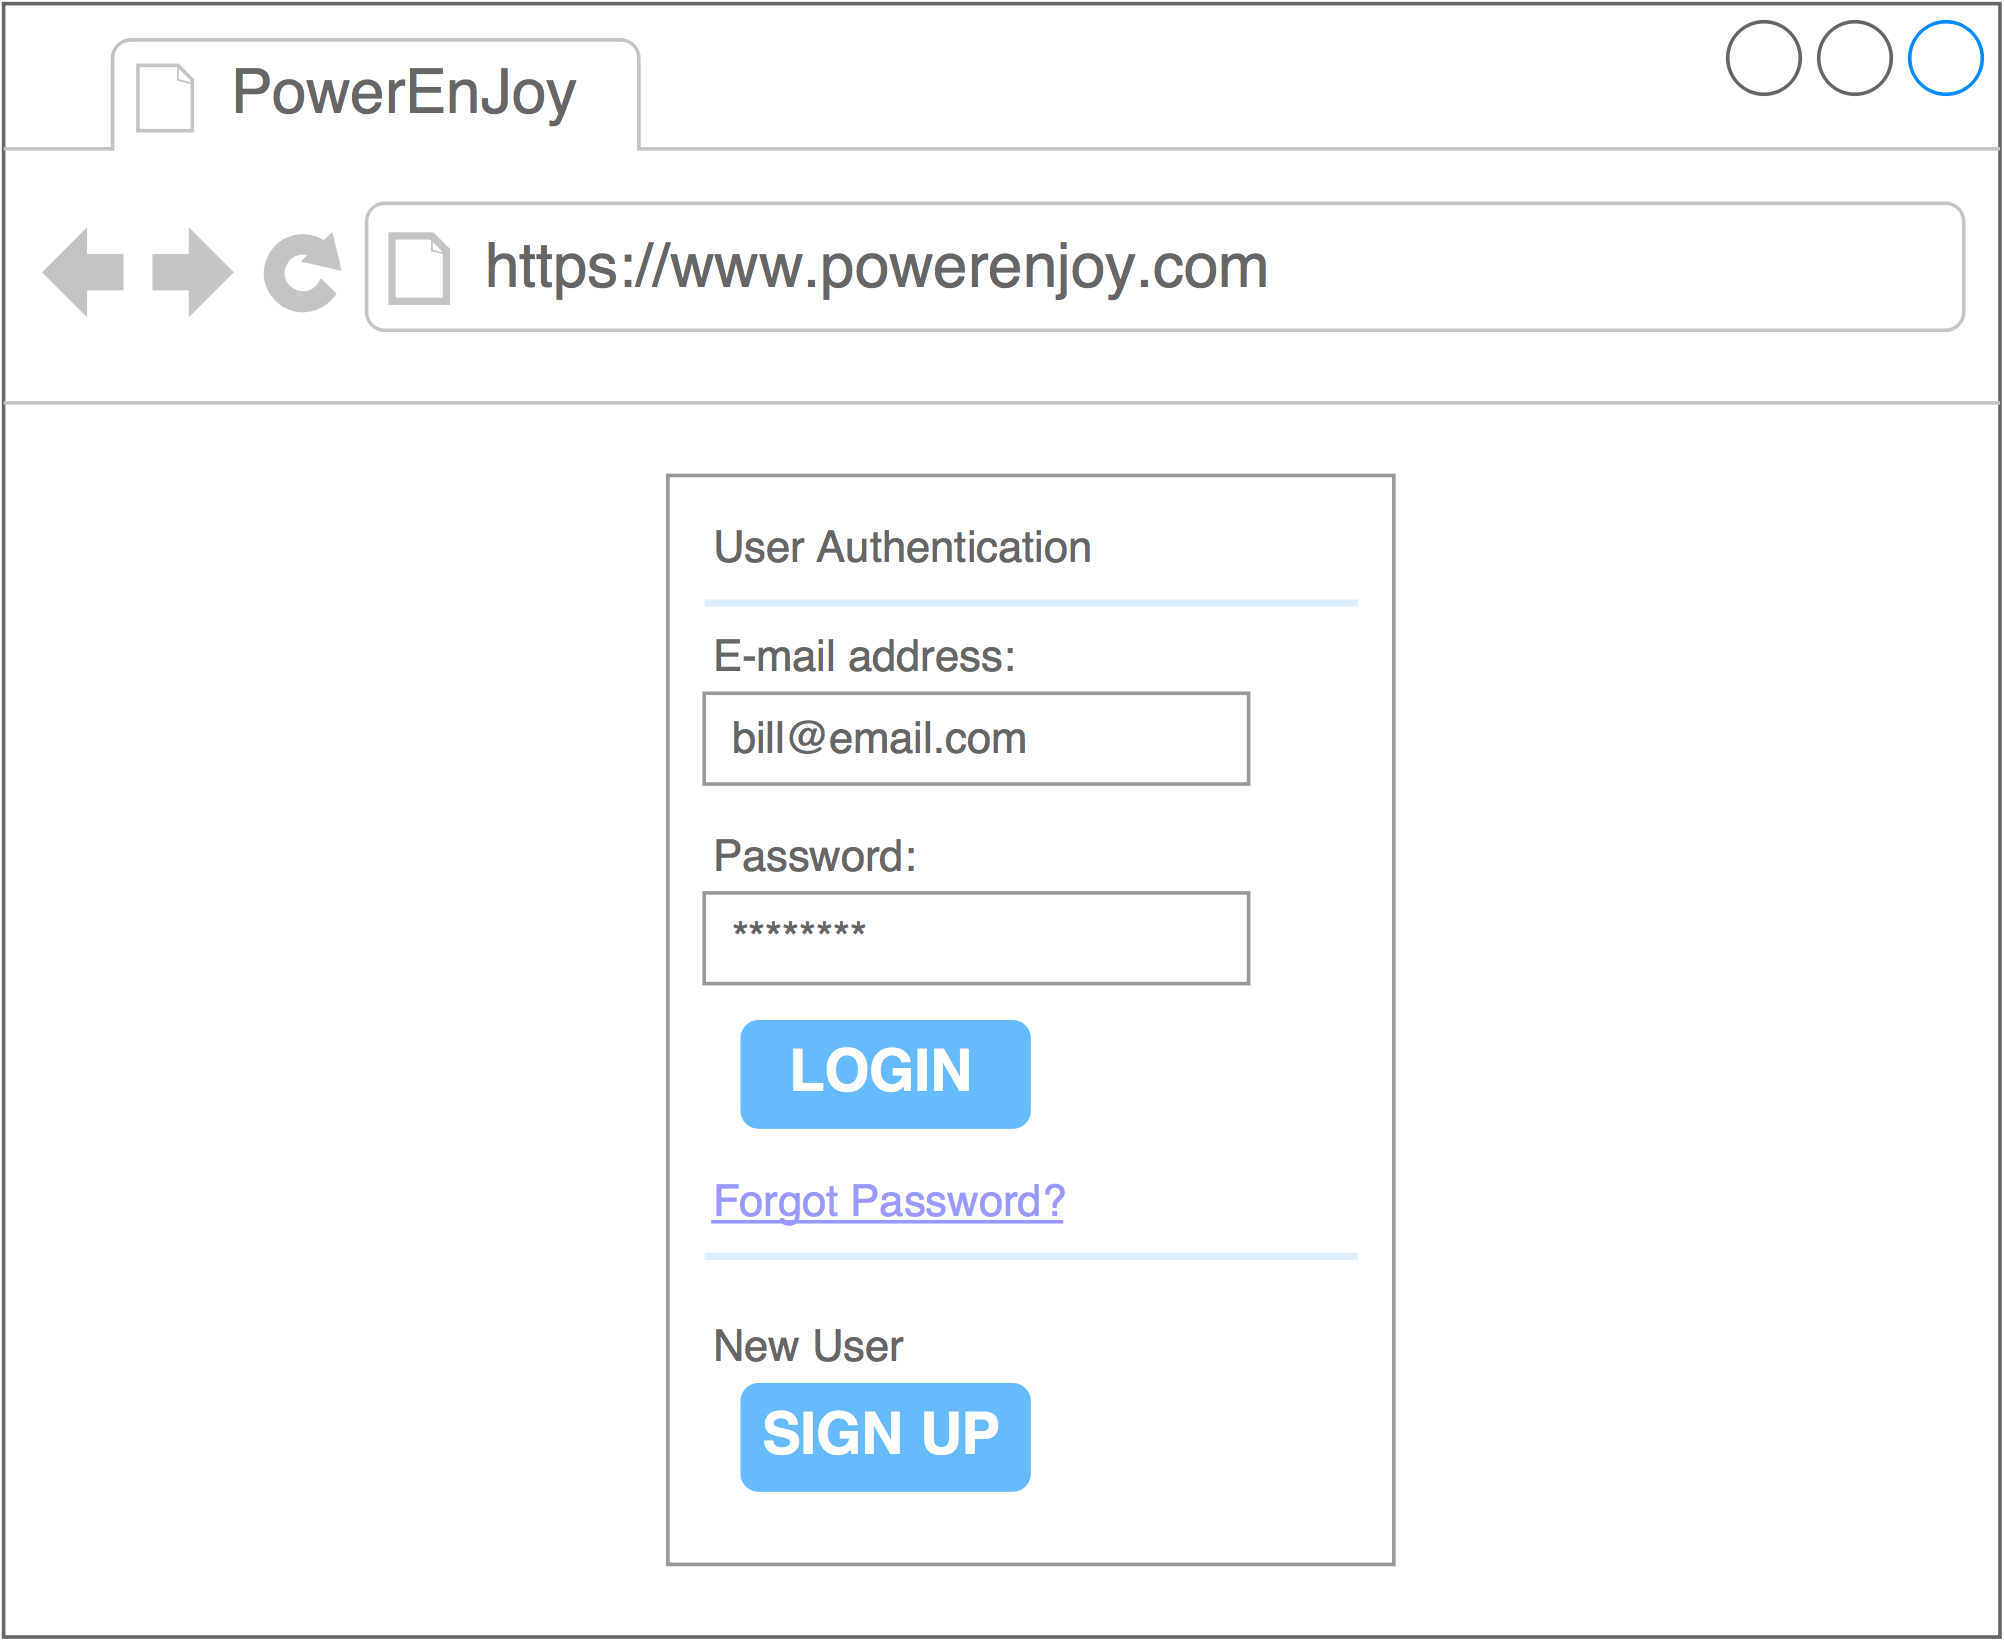
\includegraphics[width=\textwidth]{./specific_requirements/features/diagrams/web_login.png}
		\caption{Mockup of the login webpage.}
\end{center}
\end{figure}

\begin{figure}[H]
\begin{center}
		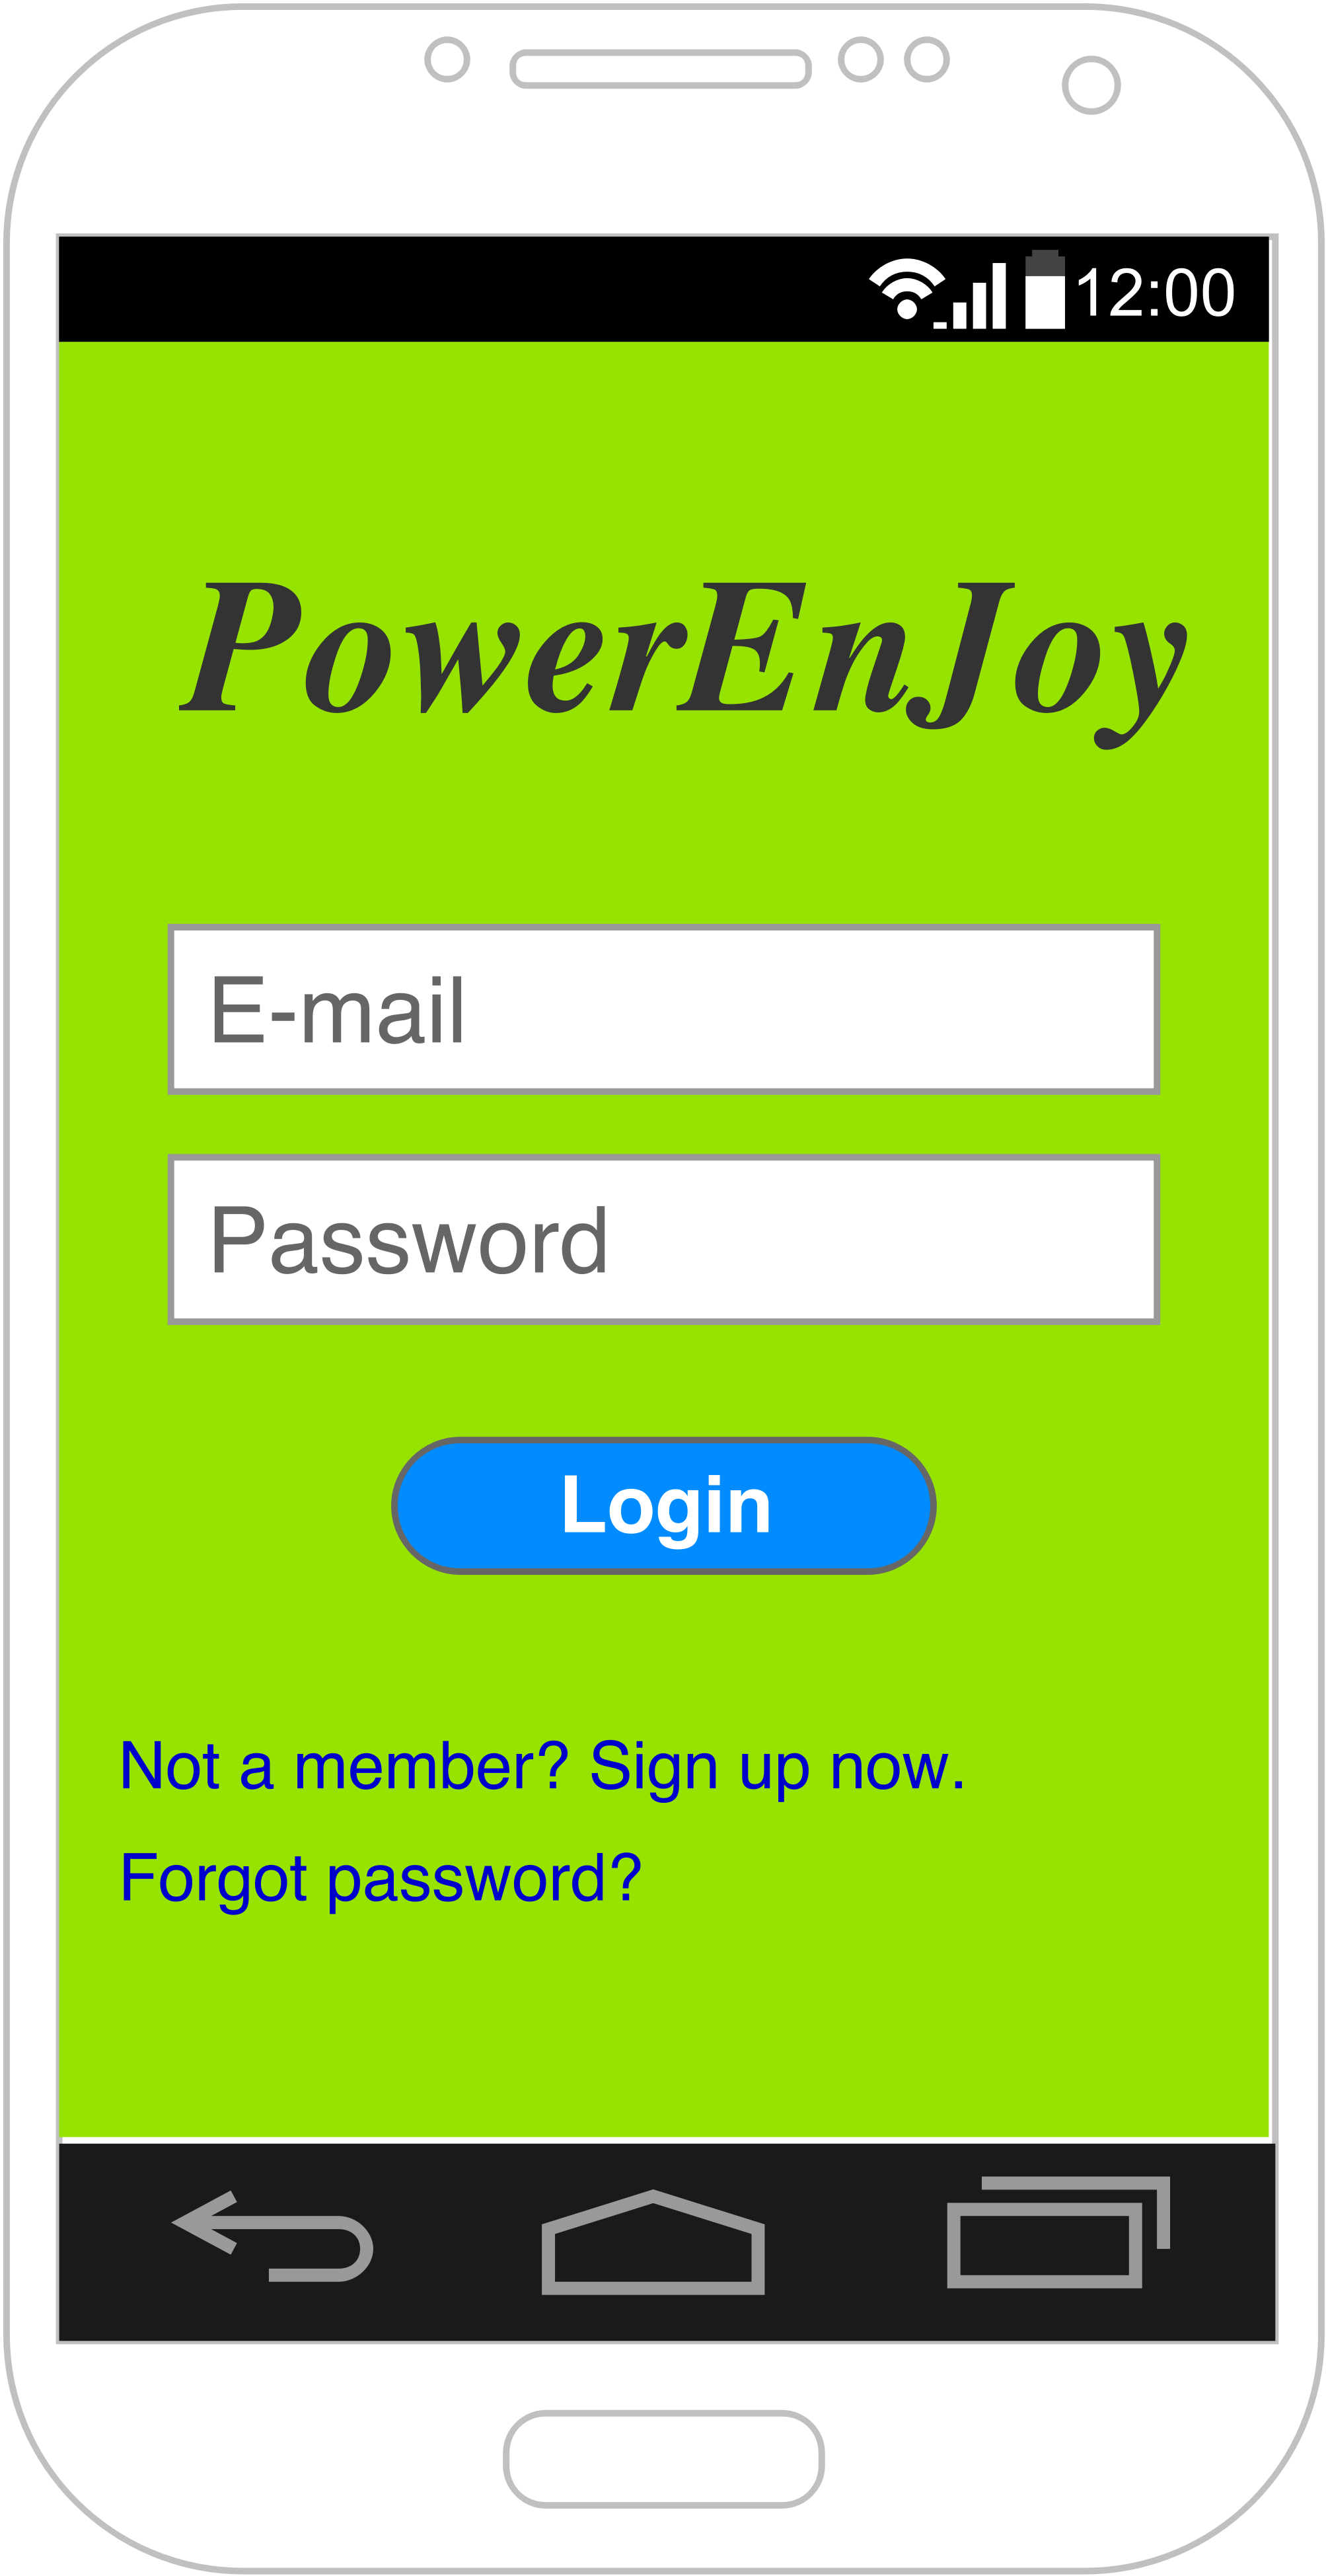
\includegraphics[width=0.4\textwidth]{./specific_requirements/features/diagrams/mobile_login.png}
		\caption{Mockup of the mobile version of the login screen.}
\end{center}
\end{figure}